%%%%%%%%%%%%%%%%%%%%%%%%%%%%%%%%%%%%%%%%%%%%%%%%%%%%%%%%%%%%%%%%%%
%%%%%%%% ICML 2016 EXAMPLE LATEX SUBMISSION FILE %%%%%%%%%%%%%%%%%
%%%%%%%%%%%%%%%%%%%%%%%%%%%%%%%%%%%%%%%%%%%%%%%%%%%%%%%%%%%%%%%%%%

% Use the following line _only_ if you're still using LaTeX 2.09.
%\documentstyle[icml2016,epsf,natbib]{article}
% If you rely on Latex2e packages, like most moden people use this:
\documentclass{article}

% use Times
\usepackage{times}
% For figures
\usepackage{graphicx} % more modern
%\usepackage{epsfig} % less modern
\usepackage{subfigure} 

% qdeee: for mathbb
\usepackage{amsmath}
\usepackage{amssymb}

% For citations
\usepackage{natbib}

% For algorithms
\usepackage{algorithm}
\usepackage{algorithmic}

% For sub-files
\usepackage{standalone}

\usepackage{multicol}
\usepackage{multirow} % http://ctan.org/pkg/multirow
\usepackage{hhline} % http://ctan.org/pkg/hhline

% For plots
\usepackage{epstopdf}
%\usepackage{color}

% As of 2011, we use the hyperref package to produce hyperlinks in the
% resulting PDF.  If this breaks your system, please commend out the
% following usepackage line and replace \usepackage{icml2016} with
% \usepackage[nohyperref]{icml2016} above.
\usepackage{hyperref}

% Packages hyperref and algorithmic misbehave sometimes.  We can fix
% this with the following command.
\newcommand{\theHalgorithm}{\arabic{algorithm}}

% Employ the following version of the ``usepackage'' statement for
% submitting the draft version of the paper for review.  This will set
% the note in the first column to ``Under review.  Do not distribute.''
\usepackage{icml2017} 

% Employ this version of the ``usepackage'' statement after the paper has
% been accepted, when creating the final version.  This will set the
% note in the first column to ``Proceedings of the...''
% \usepackage[accepted]{icml2017}


% The \icmltitle you define below is probably too long as a header.
% Therefore, a short form for the running title is supplied here:
\icmltitlerunning{Using Matrix Factorization Methods for Multiclass Classification tasks}

\begin{document} 

\twocolumn[
\icmltitle{Using Matrix Factorization Methods for Multiclass Classification Tasks}
            

% It is OKAY to include author information, even for blind
% submissions: the style file will automatically remove it for you
% unless you've provided the [accepted] option to the icml2017
% package.

% list of affiliations. the first argument should be a (short)
% identifier you will use later to specify author affiliations
% Academic affiliations should list Department, University, City, Region, Country
% Industry affiliations should list Company, City, Region, Country

% you can specify symbols, otherwise they are numbered in order
% ideally, you should not use this facility. affiliations will be numbered
% in order of appearance and this is the preferred way.
\icmlsetsymbol{equal}{*}

\begin{icmlauthorlist}
\icmlauthor{Ruslan Solovev}{equal,to}
\icmlauthor{Igor Kuralenok}{equal,to,goo}
\end{icmlauthorlist}

\icmlaffiliation{to}{University of Torontoland, Torontoland, Canada}
\icmlaffiliation{goo}{Googol ShallowMind, New London, Michigan, USA}

\icmlcorrespondingauthor{Ruslan Solovev}{solovevr@gmail.com}
\icmlcorrespondingauthor{Igor Kuralenok}{ikuralenok@gmail.com}


% You may provide any keywords that you 
% find helpful for describing your paper; these are used to populate 
% the "keywords" metadata in the PDF but will not be shown in the document
\icmlkeywords{multinomial logistic regression, matrix factorization, gradient boosting}

\vskip 0.3in
]

% this must go after the closing bracket ] following \twocolumn[ ...

% This command actually creates the footnote in the first column
% listing the affiliations and the copyright notice.
% The command takes one argument, which is text to display at the start of the footnote.
% The \icmlEqualContribution command is standard text for equal contribution.
% Remove it (just {}) if you do not need this facility.

\printAffiliationsAndNotice{}  % leave blank if no need to mention equal contribution
%\printAffiliationsAndNotice{\icmlEqualContribution} % otherwise use the standard text.
%\footnotetext{hi}

\begin{abstract} 
In this paper we introduce a new approach to multiclassification based on simultaneous build of all scoring functions in multinomial logistic regression framework. The proposed algorithm provides more lightweight decision function while being on par with state-of-the-art methods in terms of prediction quality. The method is based on multinomial logistic regression and gradient boosting. The first part allows the researcher not to bother balancing of different classes in dataset, and the second give her the opportunity to control the time to model quality ratio.
\end{abstract} 

\section{Introduction}
\label{introduction}
Classification onto more than two classes is very natural setting for many tasks. Among others we should mention text classification, object recognition, protein folds etc. There are four principal approaches to this problem known from the literature: one-vs-rest, multinomial logistic regression \cite{GLM}, multiclass boosting \cite{journals/jmlr/MukherjeeS13} and using complex system of binary classifiers with associated modeling matrix \cite{Allwein00reducingmulticlass}.

Each of these families have their properties and depending on the task could be more or less effective. The simplicity of one vs. rest makes it the most popular method in everyday work of ML practician. On the other hand this simplicity in training process is balanced by need of balancing the result scoring functions either by count of the representatives of each class or by other methods. Multinomial logistic regression based methods are the opposite extreme case. They are much easier to prepare for learning---scoring functions will be comparable by the design, but it takes ages to learn a strong model. Multiclass boosting allows us to split this process building one weak classifier at a time balancing the weights of examples, but we still need to solve multi-classification problem on each step. Modeling matrix approach generalize the one-vs-rest allowing one to build binary classifiers complimentary to each other. This way allows us to build smaller number of decision functions than the $K-1$, where $K$ is number of classes. There are some works about the building of the modeling matrix \cite{Zhao_sparseoutput, modelmatrix2}, however there is no good way to build this matrix universally and it should be constructed in ad-hoc manner in most of the cases.

Our goal is to combine described approaches to get the method that is as simple as one-vs-rest, able to work with lot of classes, less sensitive to class imbalance, has light decision function to be used online. To achieve these properties we do the gradient boosting for multinomial logistic regression to find a decision function in form of single ensemble. The multinomial logistic regression particularly allows us to forget about class imbalance; gradient boosting allows one to control the time to model quality ratio; and the simplicity of the decision function allows us to convert multi-classification into series of regression tasks.

% The fo

% Our contribution as follows:
% \begin{itemize}
% \item We propose the GradFac multiclassification algorithm that is based on gradient boosting and matrix factorization. We show that in most cases it can reduce total count of weak models without sufficient quality degradation.
% \item We describe the main disadvantage of the new algorithm and propose two fixes: matrix columns bootstrapping and \emph{ElasticNet} factorization. 
% \item We apply the GradFac algorithm to the classic gradient boosted tree classifier on benchmark datasets.
% \end{itemize}



\section{Motivation}

Many algorithms in ML are focused around classification or regression tasks and the idea of employing them for multiclassification looks attractive. The modeling matrix approach formulated by Allwein, Schapire and Singer \cite{Allwein00reducingmulticlass} allows one to split this complex task into binary classification subtasks. Unfortunately the elements of the modeling matrix must be from set of $\{-1,0,1\}$ and this fact makes the optimization on this matrix much more difficult \cite{Zhao_sparseoutput, modelmatrix2}. We want to get rid of this limitation to simplify the optimization task. Another important property of this approach is that we can use when number of classes is significant and it is next to impossible to train scoring function for each of them. In this case we ``code'' the class by modeling matrix row and, using results of the binary classifiers, are able to estimate the this class probability.

We will look for decision function in the class of the following functions:
\begin{equation}
H_c(x) = \sum_t b_{ct} h_t(x) 
\end{equation}
where $H_c(x)$ is a scoring function for class $c$ at point $x$, $b_{ct}$ is a scalar value, associated with the class $c$ at step $t$, and $h_t(x)$ is some real-valued function of $x$. The probability of class $c$ look exactly like one in multinomial logistic regression:
\begin{equation}
  P(Y = c \arrowvert x, H) =
  \begin{cases}
    \frac{ e^{H_{c}(x)} }
       { 1+\sum_{j=1}^{K-1} e^{H_{j}(x)} }
    , & c \in \{1, \ldots, K-1 \} \\

    \frac{ 1 }
       { 1 + \sum_{j=1}^{K-1} e^{H_{j}(x)} }
    , & c=K
  \end{cases}\label{eq:MLR_model}
\end{equation}
where $P(Y = c \arrowvert x, H)$ is desired probability of the class $c \in \{1\ldots K\}$ for the query $x$.

This type of decision function look very similar to those using modeling matrix: $\mathbb{B} = \{b_{ct}\}$ form the matrix itself, and the $h_t$ are some regression task solutions:
\begin{equation}
h_{t+1} = \arg \min_h \|h(X) - r_t\|.
\end{equation}
Our task is to find proper series of $(b_t, r_t)$. We use modification of the multinomial logistic regression gradient boosting for this.

\subsection{Multinomial logistic regression}
The boosting of multinomial logistic regression is a well studied topic \cite{Friedman98additivelogistic}. The multinomial regression models discriminative surfaces between classes in form of $H_{c_1}(x)=H_{c_2}(x)$, this brings probability of the class into form of (\ref{eq:MLR_model}) \cite{GLM}. The boosting approach implies the ensemble form of scoring function $H_c(x) = \sum h_{ct}(x)$. The target function is the following:
\begin{multline*}
	L(X\arrowvert H) = \sum_{(x,y) \in X} \log P(Y = y \arrowvert x, H) = \\
	= \sum_{(x,y) \in X} \log \frac{ I\{y \ne K \}e^{H_y(x)} + I\{y=K\} }{ 1+\sum_{c=1}^{K-1} e^{H_c(x)} }
\end{multline*}
in this case $X$ is not only features matrix, but entire set of $(x, y)$ precedents. On each step we want $h_{t + 1}(X)$ to be aligned with the $\frac{\partial L(X|H)}{\partial H_c(x)}(H_t(X))$. For simplicity one can interpret $\frac{\partial L(X|H)}{\partial H_c(x)}(H_t(X))$ as a matrix $R_t$ of size $|X|\times K-1$. Then it is time to optimize $h_{ct+1}$:
\begin{equation}
h_{ct+1} = \arg \min_h \|h_c(X) - r_{ct}\|
\label{eq:MLR_boosting_step}
\end{equation}
where $r_c$ is a column of the matrix representation of gradient $R$. At this step we need to build the regression $K-1$ times and this part is the most computationally intensive. We have described the independent variant of the optimization, but it can be enhanced even further by dropping the independence assumption for certain types of decision functions (such as regression trees).

\subsection{The idea of FMCB}
The main difference from the multinomial regression boosting is the form of decision function. We want to simultaneously optimize (\ref{eq:MLR_boosting_step}) for all classes. But the $l_2$ target function is additive and we can rewrite the optimization in the following form:
\begin{equation}
(h_{t+1},b_{t+1}) = \arg \min_{h,b} \sum_c \|b_ch(X) - r_{ct}\|
\end{equation}
where $b_{t+1}$---column of the future modeling matrix. At this point we assume that this optimization could be split into two steps:
\begin{equation}\begin{array}{l}
(b_{t+1},r_{t+1}) = \arg \min_{b,r} \|b r^T - R_t\|_F \\
h_t	= \arg \min_{h} \|h(X) - r_{t+1}\|
\end{array}\end{equation}
According to the Eckart-Young-Mirsky theorem \cite{Eckart1936} there is exact solution of the first optimization. The second one is just a regression problem. The split assumption is correct when $h$ is flexible enough to bring the $\|h(X) - r_{t+1}\|$ to zero. In most of the cases this is not true and this step won't allow us to use results of the boosting convergence analysis \cite{??}. In the next section

\section{Factorized MultiClass Boosting}
The proposed algorithm optimizes the likelihood function:
\begin{multline*}
	L(X\arrowvert H) = \sum_{(x,y) \in X} \log \frac{ I\{y \ne K \}e^{H_y(x)} + I\{y=K\} }{ 1+\sum_{c=1}^{K-1} e^{H_c(x)} }.
\end{multline*}
The decision takes form of vector function:
\begin{equation}
H(x) = \sum_t b_{t} h_t(x) 
\end{equation}
where $b_t$ are vectors of $K-1$ components and $h_t$ are real functions of $x$. The optimization is done iteratively. $H_c(x)$ are treated as independent variables and therefor one can get gradient of target function in terms of these variables. It is possible to present this gradient vector as a matrix each column of this matrix presents gradient vector of the appropriate class scoring function:
\begin{equation}
\nabla L = 
\left(
\begin{array}{ccc}
	  \frac{ \partial L }{ \partial H_{1}(x_{1}) } 
	& \cdots 
	& \frac{ \partial L }{ \partial H_{K-1}(x_{1}) } \\

	  \vdots & \ddots & \vdots\\

	  \frac{ \partial L }{ \partial H_{1}(x_{|X|}) } 
	& \cdots 
	& \frac{ \partial L }{ \partial H_{K-1}(x_{|X|}) }
\end{array}
\right)_{|X| \times (K-1)}
\end{equation}
Each step of optimization is done as close to the $R_t = \nabla L(H_t(X))$ as possible. To do so we factorize the matrix form of the gradient $R$ by rank $1$ matrix $b h(X)^T$ using Frobenius distance as the metric:
\begin{equation}
(b_{t+1},r_{t+1}) = \arg \min_{b,r} \|b r^T - R_t\|_F
\label{eq:factorization_step}
\end{equation}

According to the Eckart-Young-Mirsky theorem \cite{Eckart1936}, solving (\ref{eq:factorization_step}) means finding the left and the right singular vectors of $R_t$ associated with the largest singular value of $R_t$. Therefore, one may apply the following algorithm: 
\begin{enumerate}
	\item Evaluate the singular decomposition of gradient's matrix: $R = U \Sigma V^T$
	\item Take the largest singular value $\sigma_{1}$ and associated singular vectors $u$ and $v$.
	\item Return $\overline{u}={\sigma_{1}}{\Vert v \Vert}_{2}u$ and $\overline{v}=\frac{1}{\Vert v \Vert}_{2}v$ as solution.
\end{enumerate}
However, experiments show that starting from the some iteration, singular values become too close to each other and choice of singular vectors associated with the largest singular value becomes non-trivial. It leads to factorization error growth because the single pair of the left and the right singular vectors is no longer meaningful characteristic of the matrix. We call this negative effect "the spreading of singular values", as the matrix is spreading across several pairs of singular vectors. To overcome this difficulty we have introduced the bias on each step. In the following chapters we will implement the bias in form of prior (and appropriate regularization) and introduction of the noise into data.

From the solutions family we choose the pair where $\|b_{t+1}\| = 1$. To find the decision ensemble term $h_{t+1}$ we minimize the distance with factorization component $r_{t+1}$:
\begin{equation}
h_{t+1}	= \arg \min_{h} \|h(X) - r_{t+1}\|
\label{eq:minimization_step}
\end{equation}
For our experiments we have used modification of the CART algorithm for oblivious trees \cite{Gulin_winningthe} at this step.

\subsection{Regularization}
Instead of solving (\ref{eq:factorization_step}), consider the next problem:
\begin{multline}
	u^{*}, v^{*} = \arg\min_{u,v}\sum_{i,j}\left(\nabla L_{ij}-u_{i}v_{j}\right)^{2} + \\
	+\alpha_{1} \Vert u\Vert_{1} + \alpha_{2} \Vert u\Vert_{2}^{2} 
	+\beta_{1}  \Vert v\Vert_{1} + \beta_{2}  \Vert v\Vert_{2}^{2}. \label{eq:def-argmin-elasticnet}
\end{multline}
Added terms are called \emph{Elastic-Net regularization} for (\ref{eq:mx_approx}) \cite{elasticnet05}. Usually similar problems are considered for non-negative matrix factorization \cite{MahNMF},\cite{another-nmf-with-en}, however we don't need such constraint.

We employ alternating iterations idea [ref to ALS] for solving (\ref{eq:def-argmin-elasticnet}). For example, consider (\ref{eq:def-argmin-elasticnet}) with fixed $\overline{v}$. Then:
\begin{multline*}
	u^{*} = \arg\min_{u}\sum_{i,j}\left(\nabla L_{ij}-u_{i}\overline{v}_{j}\right)^{2} + \\
	+ \alpha_{1}\Vert u\Vert_{1}+\alpha_{2}\Vert u\Vert_{2}^{2}
	+ \beta_{1}\Vert\overline{v}\Vert_{1}+\beta_{2}\Vert\overline{v}\Vert_{2}^{2} = \\
	= \arg\min_{u}\sum_{i,j}\left(\nabla L_{ij}-u_{i}\overline{v}_{j}\right)^{2}
	+ \alpha_{1}\Vert u\Vert_{1}+\alpha_{2}\Vert u\Vert_{2}^{2}
	\label{eq:elastic-net-argmin}
\end{multline*}
Therefore, we have reduced the source problem to the linear regression problem with \emph{Elastic-Net} regularization. Indeed, we can rewrite it in canonical form:
 \begin{equation*}
x^{*}=\arg\min\Vert y-Ax\Vert_{2}^{2}+\alpha_{1}\Vert x\Vert_{2}^{2}+\alpha_{2}\Vert x\Vert_{1},\label{eq:elastic-net-canon-argmin}
\end{equation*}
where $A \in \mathbb{R}^{N(K-1)\times N}$ and $y \in \mathbb{R}^{N(K-1)}$:
\[
A =
\begin{pmatrix}
	v_{1}     		& 				&		  \\
	\vdots			& \mathbb{O}  	&		  \\
	v_{K-1}			& 				&		  \\
					& \ddots		&		  \\
					&   			& v_{1}	  \\
					& \mathbb{O}	& \vdots  \\
					& 				& v_{K-1}
\end{pmatrix},
y=\begin{pmatrix}\begin{array}{l}
	\nabla L_{1,1}		\\
	\vdots				\\
	\nabla L_{1,K-1}	\\

	\vdots				\\
	
	\nabla L_{N,1}		\\
	\vdots				\\
	\nabla L_{N,K-1}
\end{array}\end{pmatrix}
\]
Detailed algorithm for \emph{Elastic-Net} problem could be found at \cite{elasticnet05} or \cite{Hastie_theelements}. 

Similarly, one could derive the linear system in case of fixed vector $u$. Hence, the final algorithm is similar to ALS but instead of alternating gradient steps one needs to alternate solving \emph{Elastic-Net} problem. Due to the simple structure of matrix $A$, these problems could be solved very efficiently.

\begin{figure}
\vskip 0.2in
\begin{center}
\centerline{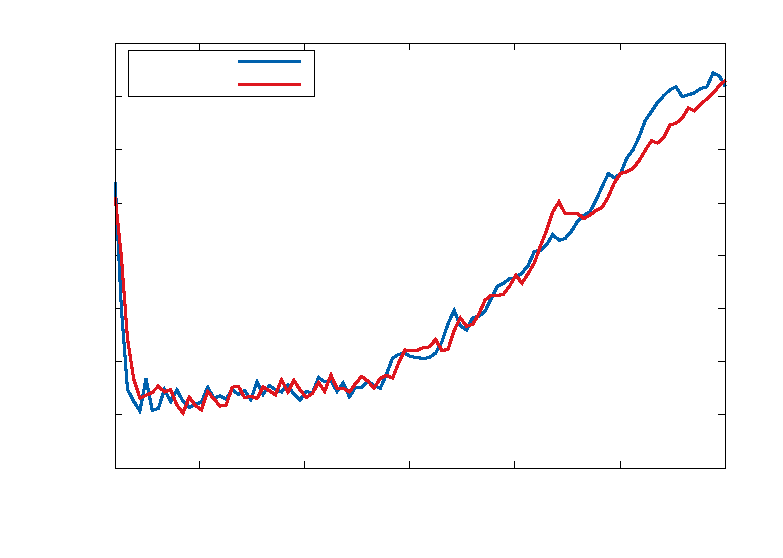
\includegraphics[width=\columnwidth]{figures/cn.tex}}
\caption{Condition number of the gradient matrix during training GF and GFEN models on \emph{segmentation} dataset.}
\end{center}
\vskip -0.2in
\end{figure}

\subsection{Columns bootstrapping}
We employ statistical bootstrap idea \cite{Efron1992bootstrap}. On each iteration we assign random integer weights to columns of the gradient's matrix. It ensures that singular values will be "shake-up" and consequently it particularly protects us from the problem described above. Required weights could be generated by discrete random variable $\xi$ that has a Poisson distribution with $\lambda = 1$. Due to the fact that $\mathbb{E} \xi = 1$, this weighing approach has a simple physical meaning: in the most of cases we consider all columns of the gradient's matrix but sometimes we amplify ($\xi > 1$) or mute ($\xi = 0$) some of them.







\section{Stop}

\section{Multinomial logistic regression}
In this section we consider application of gradient boosting algorithm to the multinomial logistic regression problem. This application was well described by Friedman \yrcite{Friedman98additivelogistic}, so we just reformulate already known.

Assume we have a training instances set $D={(x^i, y^i)}_{i=1}^N$,  where $x\in\mathbb{R}^n$ is an instance's feature vector
and $y\in\left\{ 1,\dots,K\right\} $ is an instance's class label. According the multinomial regression model definition \cite{GLM}, we need to build the decision in the next probabilistic form:
\begin{equation}
	\mathbb{P}(Y = c \arrowvert x) =
	\begin{cases}
		\frac{ e^{s_{c}(x)} }
			 { 1+\sum_{j=1}^{K-1} e^{s_{j}(x)} }
		, & c \in \{1, \ldots, K-1 \} \\

		\frac{ 1 }
			 { 1 + \sum_{j=1}^{K-1} e^{s_{j}(x)} }
		, & c=K
	\end{cases}\label{eq:MLR_model}
\end{equation}
Here $s_{j}(x), j \in \{ 1, \ldots, K-1 \}$ are real functions (a.k.a. \textit{scoring functions}) of some class $\mathbb{F}$:
\[
	s_{j}(x): \mathbb{R}^{n} \rightarrow \mathbb{R}, j=1, \dots, K-1.
\]
Note that final decision function is fully determined by these functions.
Consider corresponding log-likelihood function for (\ref{eq:MLR_model}):
And the problem is formulated as follows: find $K-1$ functions $s_{1}^{*}(x),\dots,s_{K-1}^{*}(x)$ of class $\mathbb{F}$ such that
\begin{equation}
(s_{1}^{*}, \dots, s_{K-1}^{*}) = \arg\max_{s_{j} \in \mathbb{F}} L(s_{1},\dots,s_{K-1}\arrowvert X).\label{eq:argmaxL}
\end{equation}

We employ gradient boosting for solving (\ref{eq:argmaxL}).
Note that with fixed functions $s_1,\ldots,s_{K-1}$ target function $L$ becomes a $N\times(K-1)$ multivariate function of $s_1(x_1),\ldots,s_{K-1}(x_N)$ variables. Consider the gradient\footnote{Formally, the matrix notation for partial derivatives is reserved by Jacobian. We use the gradient's matrix notation for the convenience here.} of that function:
\[
\nabla L = 
\left(
\begin{array}{ccc}
	  \frac{ \partial L }{ \partial s_{1}(x_{1}) } 
	& \cdots 
	& \frac{ \partial L }{ \partial s_{K-1}(x_{1}) } \\

	  \vdots & \ddots & \vdots\\

	  \frac{ \partial L }{ \partial s_{1}(x_{N}) } 
	& \cdots 
	& \frac{ \partial L }{ \partial s_{K-1}(x_{N}) }
\end{array}
\right)_{N \times (K-1)}
\]
Partial derivatives of $L$ are:
\begin{multline}
\frac{ \partial L }{ \partial s_{j}(x_{i}) }=
\frac{ \partial L(s_{1}(x_{i}),\dots,s_{K-1}(x_{i})) }{ \partial s_{j}(x_{i}) }= \\ =
\frac{ e^{s_{j}(x_{i})} }{ 1+\sum_{k=1}^{K-1} e^{s_{k}(x_{i})} } - I\{y_{i} = j\} \label{eq:partial_L}
\end{multline}
According the gradient boosting algorithm, on each iteration we have to train a L2-approximation of gradient of the target function. Therefore, we have to train $K-1$ approximation models: one  model per each column of the gradient matrix. See Algorithm~\ref{alg:boost_mlr} for details.


\begin{algorithm}[tb]
   \caption{Gradient boosting for MLR}
   \label{alg:boost_mlr}
\begin{algorithmic}
   \STATE {\bfseries Input:} step $\alpha$, iterations count $T$.
   \STATE $H^{(0)}(x):= \mathbb{O} \in \mathbb{F}^{K-1}$ \COMMENT{initial zero model}
   \STATE $\overline{x}^{(0)} := \mathbb{O} \in \mathbb{R}^{N \times (K-1)}$ \COMMENT{initial cursor}

   \FOR{$t=1$ {\bfseries to} $T$}
   		\STATE Evaluate $\nabla L$ at $\overline{x}^{(t-1)}$ using (\ref{eq:partial_L}).
   		\FOR{$j=1$ {\bfseries to} $K-1$}
   			\STATE Train weak model $h_{j}^{(t)}(x)$ using $\{X,\nabla L^{[j]}\}$ as a training set and MSE as a target function:
   			\[
				h_{j}^{(t)}(x)=\arg\min_{h \in \mathbb{F}} \sum_{i=1}^{N}\left(\nabla L_{ij}-h(x_{i})\right)^{2}
			\]
		\ENDFOR
		\STATE Update model: $H^{(t)}(x)=H^{(t-1)}(x)+\alpha h^{(t)}(x)$.
		\STATE Update cursor: $\overline{x}^{t} = \overline{x}^{(t-1)} + h^{(t)}(X)$.
   \ENDFOR
   
\end{algorithmic}
\end{algorithm}


\section{GradFac}

\subsection{Motivation}
We will look for decision function in the class of the following functions:
$$
H_c(x) = \sum_t b_{ct} h_t(x) 
$$
where $H_c(x)$ is a scoring function for class $c$ at point $x$, $b_c$ is scalar value, associated with the class $c$ at step $t$, and $h_t(x)$ is some real-valued function of $x$. The probability of class $c$ will look exactly like one in multinomial logistic regression:
\begin{equation}
  P(Y = c \arrowvert x, H) =
  \begin{cases}
    \frac{ e^{H_{c}(x)} }
       { 1+\sum_{j=1}^{K-1} e^{H_{j}(x)} }
    , & c \in \{1, \ldots, K-1 \} \\

    \frac{ 1 }
       { 1 + \sum_{j=1}^{K-1} e^{H_{j}(x)} }
    , & c=K
  \end{cases}
\end{equation}
This type of decision function look very similar to those using modeling matrix, the difference is that we use real values instead of those from $\{-1,0,1\}$ set in modeling matrix $\mathbb{B} = \{b_{ct}\}$ and will build regression on each step instead of classification.

To build a sequence of $b_t$ and $h_t$ we use the idea of Friedman's gradient boosting. The target function we use is likelihood of the data based on introduced probability $P(Y = c \arrowvert x, H)$:
$$
\hat{H}(x) = \arg \min_H \sum_{(x,y) \in X} \log P(Y = c \arrowvert x, H)
$$
where $(x,y)$ is an example coming from training set $X$, $H$---vector of size $k-1$. On each step we build a weak model $(b_t, h_)$ to be as close to likelihood gradient matrix $\frac{\partial L}{\partial H_c(x)}\left(X\right)$ as possible:

$$
(b_t, h_t) = \arg \min_{b,h} \left\|\frac{\partial L}{\partial H_c(x)}\left(X\right) - b_t h_t(X)\right\|_F
$$


%Unfortunately in this case we are unable to use direct factorization of the gradient matrix. With each step the condition number of the matrix will lower because the step $b_t h_t(x)$ is close to major eigen vector. Reduction of the condition number will lower the effectiveness of factorization with each step. To overcome this difficulty we have introduced the bias on each step. In the following chapters we will implement the bias in form of prior (and appropriate regularization) and introducion of the noise into data.





% In the previous section we have shown the application of gradient boosting method to the multinomial logistic regression problem. One of the main disadvantages of this approach is model complexity. For example, if one is solving the multiclass problem with $K$ classes using gradient boosting with $T$ iterations, then total model count will be equal to $T \times (K-1)$. In practice, the number of boosting iterations is measured in thousands [cite YetiRank]. Consequently, in case of the problem with 100 classes total weak models count will be measured in hundreds of thousands.

\subsection{Main idea}
Algorithm~\ref{alg:boost_mlr} allows to build an approximation of the gradient's matrix as the set of $h_j(x)$ functions:
\[
	\nabla L \approx
	\begin{pmatrix}
		h_{1}(x_{1}) & \cdots & h_{K-1}(x_{1}) \\
			  \vdots & \ddots & \vdots \\
		h_{1}(x_{N}) & \cdots & h_{K-1}(x_{N})
	\end{pmatrix}_{N\times(K-1)}
\]

We employ matrix factorization to reduce the set of functions to the single function. Consider rank-1 approximation of the $\nabla L$ matrix:
\[
	\nabla L \approx \overline{u} \, \overline{v}^{T}, u \in \mathbb{R}^{N},v \in \mathbb{R}^{K-1},
\]
where
\begin{equation}
	\overline{u},\overline{v} =
	\arg\min_{u, v} \sum_{i,j}(\nabla L_{ij}-uv)^{2}. \label{eq:mx_approx}
\end{equation}
Given the real vector $\overline{u}$, we can train weak model on that:
\[
	u(x) = \arg\min_{u \in \mathbb{F}} \sum_{i=1}^{N}\left(\overline{u}_i-u(x_{i})\right)^{2}.
\]
Desired functions $h_{1}(x),\dots,h_{K-1}(x)$ could be expressed as a product of $u(x)$ and corresponding j-th element of the constant vector $\overline{v}$:
\[
h_{j}(x)=u(x)\cdot\overline{v}_{j}.
\]
Therefore, the actual gradient's matrix approximation could be written as follows:
\[
	\nabla L \approx
	\begin{pmatrix}
		u(x_{1})\cdot\overline{v}_{1} & \cdots & u(x_{1})\cdot\overline{v}_{K-1} \\
							   \vdots & \ddots & \vdots \\
		u(x_{N})\cdot\overline{v}_{1} & \cdots & u(x_{N})\cdot\overline{v}_{K-1}
	\end{pmatrix}_{N\times(K-1)}
\]
Now we can rewrite the weak models training stage in Algorithm~\ref{alg:boost_mlr}:
\begin{enumerate}
\item Factorize the gradient's matrix:
\[
\overline{u},\overline{v} = \arg\min_{u,v}\sum_{i,j}(\nabla L_{ij}-u_{i}v_{j})^{2}.
\]

\item Train a weak model on the vector $\overline{u}$: \label{eq:u_train}
\begin{equation}
	u(x)=\arg\min_{u\in F}\sum_{i=1}^{N}\left(\overline{u}-u(x_{i})\right)^{2}.
\end{equation}

\item Compose vector function $h(x)$:
\[
	h(x) =
	(u(x)\cdot\overline{v}_{1},\dots,u(x)\cdot\overline{v}_{K-1})=u(x)\overline{v}.
\]
\end{enumerate}
Note that (\ref{eq:mx_approx}) may be effectively solved by ALS\cite{Hu08collaborativefiltering}.


\subsection{Matrix factorization}
(This problem could be efficiently solved by \emph{alternating least squares} method \cite{Hu08collaborativefiltering}.)

According to the Eckart-Young-Mirsky theorem \cite{Eckart1936}, solving (\ref{eq:mx_approx}) means finding the left and the right singular vectors of $\nabla L$ associated with the largest singular value of $\nabla L$. Therefore, one may apply the next algorithm for solving this problem: 
\begin{enumerate}
	\item Evaluate the singular decomposition of gradient's matrix: $\nabla L = U \Sigma V^T$
	\item Take the largest singular value $\sigma_{1}$ and associated singular vectors $u$ and $v$.
	\item Return $\overline{u}={\sigma_{1}}{\Vert v \Vert}_{2}u$ and $\overline{v}=\frac{1}{\Vert v \Vert}_{2}v$ as solution.
\end{enumerate}
However, experiments show that starting from the some iteration, singular values become too close to each other and choice of singular vectors associated with the largest singular value becomes non-trivial. It leads to factorization error growth because the single pair of the left and the right singular vectors is no longer meaningful characteristic of the matrix. We call this negative effect "the spreading of singular values", as the matrix is spreading across several pairs of singular vectors.
To deal with this effect we propose two methods: regularized factorization and columns bootstrap.


\section{Discussion}
The main advantage of the \emph{GradFac} algorithm is the independence of the number of classes on the training stage: it's only required to train a single model instead of $K-1$ models. However, factorization stage depends on the number of classes. 
Consider impact of factorization on quality of the final classification model. Obviously, matrix factorization increases total error because of replacement the whole matrix to outer product of two estimated vectors $u$ and $v$. Should we decrease the algorithm's quality on purpose? To answer this question one should remember the ability of the gradient boosting method to accumulate weak models in order to obtain the strong. Therefore, to compensate introduced error, we have to increase boosting iterations count and train some additional weak models (\emph{one} per iteration). 
Suppose $L(H_{T}(x) \arrowvert X,Y) \le \varepsilon$ is true for the source algorithm after $T_{1}$ iterations and for the \emph{GradFac} algorithm after $T_{2}$ iterations. Note that $T_{1}<T_{2}$ because we need to compensate factorization error. Also note that the source algorithm requires to train $K-1$ weak models and the \emph{GradFac} algorithm requires to train $1$ model. It's hard to say definitely which model includes less weak models count: 
\[
\begin{array}{rccc}
	\text{Iterations count:}	& T_{1} 				& <		& T_{2} \\
	\text{Weak models count:}	& T_{1}\times(K-1) 		& ??	& T_{2}
\end{array}
\]
We will come back to this issue in the experiments section.

\section{Experiments} \label{experiments}
We have tested the \emph{GradFac} algorithm with natural data from the UCI repository \cite{uciRepo}. Table \ref{datasets} shows characteristics of different datasets used.

\begin{table}[t]
\caption{Statistics for the classification datasets.}
\label{datasets}
\vskip 0.15in
\begin{center}
\begin{small}
\begin{sc}
\begin{tabular}{lrrrr}
\hline
\abovespace\belowspace
Data set & Examples & Features & Classes \\
\hline
\abovespace
wine     		& 178 	& 17 	& 3     \\
letter    		& 20000 & 16 	& 26 	\\
MNIST     		& 60000 & 785 	& 10    \\
pendigits 		& 7494 	& 21 	& 8 	\\
segmentation    & 2300 	& 23 	& 6     \\
\hline
\end{tabular}
\end{sc}
\end{small}
\end{center}
\vskip -0.1in
\end{table}

\documentclass{standalone}

\begin{document}

% what's going on here: we have 5 tables with detailed results for 4 models: mll, gf, gfen, ovr. 

% Format:
% trees	mll_scores
%		gf_scores
%		gfen_scores
%		ovr_scores
%
% where scores have format: (mf_mean+mf_std [mf_low_ci, mf_high_ci]) / (MF_mean+MF_std [MF_low_ci, MF_high_ci])
% (mf - micro_f1, MF - macro_f1)

% ./letters/table
% models	mll	gf	gfen	ovr
% 3120	(0.914822+0.005035 [0.911918, 0.917485]) / (0.915615+0.005467 [0.911969, 0.918473])
% 		(0.946169+0.005010 [0.941041, 0.948078]) / (0.946278+0.004943 [0.941958, 0.948450])
% 		(0.946777+0.001795 [0.945645, 0.947726]) / (0.947035+0.001689 [0.945966, 0.947933])
% 		(0.921943+0.005899 [0.918363, 0.925238]) / (0.922707+0.005990 [0.919316, 0.926178])

% 6240 	(0.933456+0.003572 [0.931149, 0.935462]) / (0.933770+0.003819 [0.931251, 0.935766])
% 		(0.957867+0.004170 [0.955297, 0.960067]) / (0.957763+0.004111 [0.955000, 0.959936])
% 		(0.958166+0.003105 [0.956169, 0.959777]) / (0.958205+0.002980 [0.956347, 0.959789])
% 		(0.943438+0.004180 [0.940277, 0.945539]) / (0.943637+0.004080 [0.940802, 0.945865])

% 9100 	(0.940391+0.004779 [0.937782, 0.943342]) / (0.940551+0.004921 [0.937378, 0.943559])
% 		(0.960252+0.004313 [0.957661, 0.962672]) / (0.960131+0.004205 [0.957312, 0.962447])
% 		(0.962153+0.003978 [0.959672, 0.964203]) / (0.962191+0.003894 [0.959684, 0.964345])
% 		(0.949729+0.003861 [0.947195, 0.951839]) / (0.949843+0.003851 [0.947554, 0.951811])
%
%
% ./mnist/table
% models	mll	gf	gfen	ovr
% 1300	(0.952298+0.002039 [0.950951, 0.953415]) / (0.951944+0.002199 [0.950622, 0.953087])
% 		(0.963547+0.001552 [0.962680, 0.964472]) / (0.963269+0.001584 [0.962389, 0.964150])
% 		(0.963399+0.002231 [0.962294, 0.964944]) / (0.963132+0.002305 [0.962024, 0.964707])
% 		(0.956639+0.001884 [0.955551, 0.957643]) / (0.956340+0.001933 [0.955231, 0.957387])
%
% 2600	(0.962831+0.001699 [0.962050, 0.964088]) / (0.962553+0.001814 [0.961614, 0.963935])
% 		(0.969786+0.001350 [0.968934, 0.970576]) / (0.969594+0.001367 [0.968732, 0.970388])
% 		(0.970315+0.001913 [0.969208, 0.971365]) / (0.970097+0.001961 [0.969039, 0.971306])
% 		(0.966071+0.001519 [0.965120, 0.966883]) / (0.965867+0.001573 [0.964918, 0.966798])
%
% 4000	(0.967199+0.001689 [0.966281, 0.968246]) / (0.966944+0.001746 [0.965954, 0.967985])
% 		(0.972119+0.001390 [0.971332, 0.972956]) / (0.971953+0.001411 [0.971169, 0.972880])
% 		(0.973041+0.001845 [0.972067, 0.974220]) / (0.972860+0.001919 [0.971871, 0.974137])
% 		(0.970321+0.001420 [0.969258, 0.971026]) / (0.970148+0.001494 [0.969143, 0.970938])
%
%
% ./pendigits/table
% models	mll	gf	gfen	ovr
% 1300 	(0.987849+0.003195 [0.985768, 0.989564]) / (0.987961+0.003097 [0.986129, 0.989690])
% 		(0.990757+0.003586 [0.988916, 0.993002]) / (0.990934+0.003606 [0.989115, 0.993310])
% 		(0.991691+0.002887 [0.990033, 0.993393]) / (0.991835+0.002902 [0.990155, 0.993538])
% 		(0.990381+0.002695 [0.988877, 0.992011]) / (0.990605+0.002694 [0.988918, 0.992193])

% 2600 	(0.990120+0.002764 [0.988160, 0.991515]) / (0.990199+0.002694 [0.988454, 0.991553])
% 		(0.992091+0.003515 [0.990314, 0.994505]) / (0.992210+0.003566 [0.990215, 0.994266])
% 		(0.992899+0.003129 [0.991190, 0.994921]) / (0.992982+0.003196 [0.991118, 0.994934])
% 		(0.991193+0.002202 [0.989883, 0.992503]) / (0.991387+0.002196 [0.990171, 0.992635])

% 4000 	(0.990920+0.002580 [0.989103, 0.992266]) / (0.991033+0.002504 [0.989523, 0.992301])
% 		(0.992492+0.003497 [0.990842, 0.994948]) / (0.992633+0.003522 [0.990724, 0.995013])
% 		(0.993165+0.003205 [0.991293, 0.995172]) / (0.993283+0.003266 [0.991238, 0.995244])
% 		(0.991592+0.001804 [0.990603, 0.992715]) / (0.991750+0.001847 [0.990752, 0.992981])
%
%
% ./segment/table
% models	mll	gf	gfen	ovr
% 490 	(0.980592+0.010208 [0.974959, 0.986503]) / (0.980757+0.009923 [0.975127, 0.986661])
% 		(0.983644+0.008410 [0.979058, 0.988461]) / (0.984047+0.007319 [0.979819, 0.988265])
% 		(0.985342+0.007251 [0.981135, 0.989298]) / (0.986007+0.006244 [0.982566, 0.990045])
% 		(0.977452+0.008241 [0.973425, 0.983266]) / (0.977640+0.008533 [0.973782, 0.983643])

% 1050 	(0.981906+0.008462 [0.977106, 0.987422]) / (0.982009+0.008565 [0.977393, 0.987619])
% 		(0.984063+0.007776 [0.979216, 0.988166]) / (0.984386+0.006915 [0.980569, 0.988273])
% 		(0.985749+0.007579 [0.981013, 0.989848]) / (0.986255+0.006530 [0.982097, 0.989978])
% 		(0.979655+0.008432 [0.974750, 0.984958]) / (0.979733+0.008863 [0.974777, 0.985046])

% 1750 	(0.981823+0.009336 [0.976495, 0.987683]) / (0.981843+0.009565 [0.976761, 0.987241])
% 		(0.985325+0.007602 [0.980448, 0.989503]) / (0.985692+0.006752 [0.981548, 0.989411])
% 		(0.985749+0.007579 [0.980495, 0.989627]) / (0.986255+0.006530 [0.981428, 0.989473])
% 		(0.981379+0.007905 [0.976002, 0.985521]) / (0.981574+0.008253 [0.976158, 0.985744])
%
%
% ./wine/table
% models	mll	gf	gfen	ovr
% 30	(0.948882+0.046854 [0.923803, 0.975400]) / (0.947801+0.047724 [0.921972, 0.976582])
% 		(0.947671+0.040697 [0.925487, 0.970770]) / (0.925152+0.105859 [0.810031, 0.966517])
% 		(0.931409+0.050906 [0.900136, 0.959113]) / (0.909683+0.104691 [0.813619, 0.951616])
% 		(0.944808+0.084621 [0.881960, 0.984127]) / (0.951091+0.073016 [0.892577, 0.984604])

% 60	(0.969570+0.036525 [0.943902, 0.988235]) / (0.972358+0.034144 [0.946635, 0.987293])
% 		(0.967433+0.038717 [0.940616, 0.986425]) / (0.969948+0.035840 [0.945056, 0.987754])
% 		(0.954875+0.059847 [0.909626, 0.980912]) / (0.958142+0.054466 [0.914815, 0.984109])
% 		(0.950690+0.066832 [0.899690, 0.979365]) / (0.953682+0.059857 [0.910496, 0.981186])

% 90	(0.975126+0.036504 [0.946784, 0.992593]) / (0.976593+0.034738 [0.948554, 0.992172])
% 		(0.969243+0.046068 [0.937248, 0.991534]) / (0.970620+0.043485 [0.937444, 0.989167])
% 		(0.954875+0.059847 [0.905637, 0.982066]) / (0.958142+0.054466 [0.924120, 0.984178])
% 		(0.955452+0.068638 [0.898813, 0.988889]) / (0.958565+0.061596 [0.911335, 0.986070])



\begin{table*}%[t]
\label{exp-results}
\centering
\caption{Micro-averaged $F_{1}$ scores for the multinomial logistic regression (MLR), factorized multiclass boosting (FMCB), factorized multiclass boosting with elastic-net (FMCB-EN), factorized multiclass boosting with columns sampling (FMCB-CS), One-vs-Rest (OVR) models on benchmark datasets.}
\vskip 0.15in
\begin{small}
\begin{sc}
{\renewcommand{\arraystretch}{1.2}% for the vertical padding
\begin{tabular}{|l|c|c|c|c|c|c|}
\hline
\abovespace\belowspace
Dataset		& \# Models 	& MLR & FMCB & FMCB-EN 	& FMCB-CS & OVR  \\
\hline\hline
\multirow{3}{*}{wine}
	& 30    		& 0.949 $\pm$ 0.047 		 & 0.948 $\pm$ 0.041 & 0.931 $\pm$ 0.051 & \textbf{0.956 $\pm$ 0.002} & 0.945 $\pm$ 0.085\\
	& 60	  		& \textbf{0.970 $\pm$ 0.037} & 0.967 $\pm$ 0.039 & 0.955 $\pm$ 0.060 & 0.956 $\pm$ 0.002 & 0.951 $\pm$ 0.067\\
	& 90    		& \textbf{0.975 $\pm$ 0.037} & 0.969 $\pm$ 0.046 & 0.955 $\pm$ 0.060 & 0.963 $\pm$ 0.002 & 0.955 $\pm$ 0.069\\
\hline
\multirow{3}{*}{letters}
	& 3120			& 0.915 $\pm$ 0.005 & 0.946 $\pm$ 0.005 & \textbf{0.947 $\pm$ 0.002} & 0.947 $\pm$ 0.003 & 0.922 $\pm$ 0.006\\
	& 6240	 		& 0.933 $\pm$ 0.004 & 0.958 $\pm$ 0.004 & \textbf{0.958 $\pm$ 0.003} & 0.958 $\pm$ 0.003 & 0.943 $\pm$ 0.004\\
	& 9100 			& 0.940 $\pm$ 0.005 & 0.960 $\pm$ 0.004 & \textbf{0.962 $\pm$ 0.004} & 0.961 $\pm$ 0.004 & 0.950 $\pm$ 0.004\\
\hline
\multirow{3}{*}{mnist}
	& 1300			& 0.952 $\pm$ 0.002 & 0.964 $\pm$ 0.002 			& 0.963 $\pm$ 0.002 			& \textbf{0.964 $\pm$ 0.002} & 0.957 $\pm$ 0.002\\
	& 2600			& 0.963 $\pm$ 0.002 & 0.970 $\pm$ 0.001 	& 0.970 $\pm$ 0.002 			& \textbf{0.971 $\pm$ 0.002} & 0.966 $\pm$ 0.002\\
	& 4000			& 0.967 $\pm$ 0.002 & 0.972 $\pm$ 0.001 			& 0.973 $\pm$ 0.002 	& \textbf{0.973 $\pm$ 0.002} & 0.970 $\pm$ 0.001\\
\hline
\multirow{3}{*}{pendigits}
	& 1300			& 0.988 $\pm$ 0.003 & 0.991 $\pm$ 0.004 & \textbf{0.992 $\pm$ 0.003} & 0.991 $\pm$ 0.003 & 0.990 $\pm$ 0.003 \\
	& 2600			& 0.990 $\pm$ 0.003 & 0.992 $\pm$ 0.004 & \textbf{0.993 $\pm$ 0.003} & 0.992 $\pm$ 0.003 & 0.991 $\pm$ 0.002 \\
	& 4000			& 0.991 $\pm$ 0.003 & 0.992 $\pm$ 0.003 & \textbf{0.993 $\pm$ 0.003} & 0.992 $\pm$ 0.004 & 0.992 $\pm$ 0.002 \\
\hline
\multirow{3}{*}{segmentation}
	& 490			& 	0.981 $\pm$ 0.010 & 0.984 $\pm$ 0.008 & \textbf{0.985 $\pm$ 0.007} & 0.974 $\pm$ 0.003 & 0.977 $\pm$ 0.008 \\
	& 1050			& 	0.982 $\pm$ 0.008 & 0.984 $\pm$ 0.008 & \textbf{0.986 $\pm$ 0.008} & 0.975 $\pm$ 0.004 & 0.980 $\pm$ 0.008 \\
	& 1750			& 	0.982 $\pm$ 0.009 & 0.985 $\pm$ 0.008 & \textbf{0.987 $\pm$ 0.008} & 0.975 $\pm$ 0.004 & 0.981 $\pm$ 0.008 \\
\hline
\end{tabular}
\vskip -0.1in
} % {\renewcommand{\arraystretch}{1.2}% for the vertical padding
\end{sc}
\end{small}
\end{table*}
	





\end{document}
 
\subsection{Experimental setup}
Let us remind that our main goal is minimization of the total weak models count. In each experiment we compare micro-$F_1$-score that could be reached with fixed count of weak models. 

All considered models are multinomial logistic regression models that were trained with gradient boosting method. We use oblivious decision tree with depth = 6 [ref] as a weak model. The main difference between compared models is learning method for scoring functions $h_{j}(x)$ on each iteration of the gradient boosting algorithm. We consider three learning methods:
\begin{enumerate}
	\item Multinomial logistic regression. For each j-th column of the gradient's matrix we train separate decision tree and use this tree as $h_{j}(x)$.

	\item \emph{GradFac}. Using ALS we factorize the gradient's matrix to product of two vectors $\overline{u}$ and $\overline{v}$. The scoring function $h_{j}(x)$ is expressed as a product of $u(x)$ and $\overline{v}_{j}$, where $u(x)$ is a decision tree trained on vector $\overline{u}$.

	\item \emph{GradFac} with \emph{Elastic-Net} regularization. Similar to previous, but factorization is performed via alternating of \emph{Elastic-Net} problems.
\end{enumerate}
Also we include classic one-vs-rest approach to comparison. For each class we train binary logistic regression model with gradient boosting method. Again, we use oblivious decision tree with depth = 6 as a  weak model.


\subsection{Results}
The results are presented in Table 2. Each cell contains mean and standard deviation of the micro-$F_1$-score which evaluated with 10-folds cross-validation. We find that our proposed algorithm GFEN almost always achieves the highest $F_1$-score compared to other models. Also we see that in most cases we could sufficiently reduce the weak models count for GFEN or GF methods and stay competitive with state-of-the-art methods like MLR or OVR.


\section{Conclusion}
We have introduced in this paper a new multiclassification algorithm GradFac that is based on the idea of gradient's matrix factorization. Experiments demonstrated that our algorithm allows to build up to 3 times easier model than state-of-the-art models like OVR or MLR without quality degradation. Of course, more experiments are needed to better understand applicability limits of this method, especially for tasks with large class count.

There are several avenues for future research. One of the most simple ideas - variation of considering eigen vectors count (instead of 1). GradFac is also appealing for multi-label tasks because there are several target functions for such tasks \cite{Tsoumakas07multi-labelclassification} that allow to represent their gradients as matrix and consequently allow to apply factorization techniques.

% \clearpage
% Acknowledgements should only appear in the accepted version. 
\section*{Acknowledgments} 


% In the unusual situation where you want a paper to appear in the
% references without citing it in the main text, use \nocite
%\nocite{langley00}

\nocite{Hastie_theelements}
\nocite{GLM}
\nocite{Friedman98additivelogistic}
\nocite{Friedman00greedyfunction}
\nocite{Zhao_sparseoutput}
\nocite{Allwein00reducingmulticlass}
\nocite{Crammer00onthe}
\nocite{Rifkin04indefense}
\nocite{Lee01algorithmsfor}
\nocite{Koren09matrixfactorization}
\nocite{Hu08collaborativefiltering}
\nocite{Gulin_winningthe}
\nocite{Eckart1936}
\nocite{elasticnet05}
\nocite{Efron1992bootstrap}
%\nocite{multilabel12}
\nocite{uciRepo}

\bibliography{example_paper}
\bibliographystyle{icml2017}

\end{document} 